% Options for packages loaded elsewhere
\PassOptionsToPackage{unicode}{hyperref}
\PassOptionsToPackage{hyphens}{url}
%
\documentclass[
  11pt,
  ignorenonframetext,
]{beamer}
\usepackage{pgfpages}
\setbeamertemplate{caption}[numbered]
\setbeamertemplate{caption label separator}{: }
\setbeamercolor{caption name}{fg=normal text.fg}
\beamertemplatenavigationsymbolsempty
% Prevent slide breaks in the middle of a paragraph
\widowpenalties 1 10000
\raggedbottom
\setbeamertemplate{part page}{
  \centering
  \begin{beamercolorbox}[sep=16pt,center]{part title}
    \usebeamerfont{part title}\insertpart\par
  \end{beamercolorbox}
}
\setbeamertemplate{section page}{
  \centering
  \begin{beamercolorbox}[sep=12pt,center]{part title}
    \usebeamerfont{section title}\insertsection\par
  \end{beamercolorbox}
}
\setbeamertemplate{subsection page}{
  \centering
  \begin{beamercolorbox}[sep=8pt,center]{part title}
    \usebeamerfont{subsection title}\insertsubsection\par
  \end{beamercolorbox}
}
\AtBeginPart{
  \frame{\partpage}
}
\AtBeginSection{
  \ifbibliography
  \else
    \frame{\sectionpage}
  \fi
}
\AtBeginSubsection{
  \frame{\subsectionpage}
}
\usepackage{amsmath,amssymb}
\usepackage{lmodern}
\usepackage{iftex}
\ifPDFTeX
  \usepackage[T1]{fontenc}
  \usepackage[utf8]{inputenc}
  \usepackage{textcomp} % provide euro and other symbols
\else % if luatex or xetex
  \usepackage{unicode-math}
  \defaultfontfeatures{Scale=MatchLowercase}
  \defaultfontfeatures[\rmfamily]{Ligatures=TeX,Scale=1}
\fi
\usetheme[]{metropolis}
% Use upquote if available, for straight quotes in verbatim environments
\IfFileExists{upquote.sty}{\usepackage{upquote}}{}
\IfFileExists{microtype.sty}{% use microtype if available
  \usepackage[]{microtype}
  \UseMicrotypeSet[protrusion]{basicmath} % disable protrusion for tt fonts
}{}
\makeatletter
\@ifundefined{KOMAClassName}{% if non-KOMA class
  \IfFileExists{parskip.sty}{%
    \usepackage{parskip}
  }{% else
    \setlength{\parindent}{0pt}
    \setlength{\parskip}{6pt plus 2pt minus 1pt}}
}{% if KOMA class
  \KOMAoptions{parskip=half}}
\makeatother
\usepackage{xcolor}
\newif\ifbibliography
\usepackage{color}
\usepackage{fancyvrb}
\newcommand{\VerbBar}{|}
\newcommand{\VERB}{\Verb[commandchars=\\\{\}]}
\DefineVerbatimEnvironment{Highlighting}{Verbatim}{commandchars=\\\{\}}
% Add ',fontsize=\small' for more characters per line
\newenvironment{Shaded}{}{}
\newcommand{\AlertTok}[1]{\textcolor[rgb]{1.00,0.00,0.00}{\textbf{#1}}}
\newcommand{\AnnotationTok}[1]{\textcolor[rgb]{0.38,0.63,0.69}{\textbf{\textit{#1}}}}
\newcommand{\AttributeTok}[1]{\textcolor[rgb]{0.49,0.56,0.16}{#1}}
\newcommand{\BaseNTok}[1]{\textcolor[rgb]{0.25,0.63,0.44}{#1}}
\newcommand{\BuiltInTok}[1]{\textcolor[rgb]{0.00,0.50,0.00}{#1}}
\newcommand{\CharTok}[1]{\textcolor[rgb]{0.25,0.44,0.63}{#1}}
\newcommand{\CommentTok}[1]{\textcolor[rgb]{0.38,0.63,0.69}{\textit{#1}}}
\newcommand{\CommentVarTok}[1]{\textcolor[rgb]{0.38,0.63,0.69}{\textbf{\textit{#1}}}}
\newcommand{\ConstantTok}[1]{\textcolor[rgb]{0.53,0.00,0.00}{#1}}
\newcommand{\ControlFlowTok}[1]{\textcolor[rgb]{0.00,0.44,0.13}{\textbf{#1}}}
\newcommand{\DataTypeTok}[1]{\textcolor[rgb]{0.56,0.13,0.00}{#1}}
\newcommand{\DecValTok}[1]{\textcolor[rgb]{0.25,0.63,0.44}{#1}}
\newcommand{\DocumentationTok}[1]{\textcolor[rgb]{0.73,0.13,0.13}{\textit{#1}}}
\newcommand{\ErrorTok}[1]{\textcolor[rgb]{1.00,0.00,0.00}{\textbf{#1}}}
\newcommand{\ExtensionTok}[1]{#1}
\newcommand{\FloatTok}[1]{\textcolor[rgb]{0.25,0.63,0.44}{#1}}
\newcommand{\FunctionTok}[1]{\textcolor[rgb]{0.02,0.16,0.49}{#1}}
\newcommand{\ImportTok}[1]{\textcolor[rgb]{0.00,0.50,0.00}{\textbf{#1}}}
\newcommand{\InformationTok}[1]{\textcolor[rgb]{0.38,0.63,0.69}{\textbf{\textit{#1}}}}
\newcommand{\KeywordTok}[1]{\textcolor[rgb]{0.00,0.44,0.13}{\textbf{#1}}}
\newcommand{\NormalTok}[1]{#1}
\newcommand{\OperatorTok}[1]{\textcolor[rgb]{0.40,0.40,0.40}{#1}}
\newcommand{\OtherTok}[1]{\textcolor[rgb]{0.00,0.44,0.13}{#1}}
\newcommand{\PreprocessorTok}[1]{\textcolor[rgb]{0.74,0.48,0.00}{#1}}
\newcommand{\RegionMarkerTok}[1]{#1}
\newcommand{\SpecialCharTok}[1]{\textcolor[rgb]{0.25,0.44,0.63}{#1}}
\newcommand{\SpecialStringTok}[1]{\textcolor[rgb]{0.73,0.40,0.53}{#1}}
\newcommand{\StringTok}[1]{\textcolor[rgb]{0.25,0.44,0.63}{#1}}
\newcommand{\VariableTok}[1]{\textcolor[rgb]{0.10,0.09,0.49}{#1}}
\newcommand{\VerbatimStringTok}[1]{\textcolor[rgb]{0.25,0.44,0.63}{#1}}
\newcommand{\WarningTok}[1]{\textcolor[rgb]{0.38,0.63,0.69}{\textbf{\textit{#1}}}}
\usepackage{longtable,booktabs,array}
\usepackage{calc} % for calculating minipage widths
\usepackage{caption}
% Make caption package work with longtable
\makeatletter
\def\fnum@table{\tablename~\thetable}
\makeatother
\usepackage{graphicx}
\makeatletter
\def\maxwidth{\ifdim\Gin@nat@width>\linewidth\linewidth\else\Gin@nat@width\fi}
\def\maxheight{\ifdim\Gin@nat@height>\textheight\textheight\else\Gin@nat@height\fi}
\makeatother
% Scale images if necessary, so that they will not overflow the page
% margins by default, and it is still possible to overwrite the defaults
% using explicit options in \includegraphics[width, height, ...]{}
\setkeys{Gin}{width=\maxwidth,height=\maxheight,keepaspectratio}
% Set default figure placement to htbp
\makeatletter
\def\fps@figure{htbp}
\makeatother
\setlength{\emergencystretch}{3em} % prevent overfull lines
\providecommand{\tightlist}{%
  \setlength{\itemsep}{0pt}\setlength{\parskip}{0pt}}
\setcounter{secnumdepth}{-\maxdimen} % remove section numbering
\ifLuaTeX
  \usepackage{selnolig}  % disable illegal ligatures
\fi
\IfFileExists{bookmark.sty}{\usepackage{bookmark}}{\usepackage{hyperref}}
\IfFileExists{xurl.sty}{\usepackage{xurl}}{} % add URL line breaks if available
\urlstyle{same} % disable monospaced font for URLs
\hypersetup{
  pdftitle={Análisis de la asociación espacial},
  pdfauthor={Gerardo Martín},
  hidelinks,
  pdfcreator={LaTeX via pandoc}}

\title{Análisis de la asociación espacial}
\subtitle{Correlación}
\author{Gerardo Martín}
\date{2022-06-29}

\begin{document}
\frame{\titlepage}

\begin{frame}{Intro}
\protect\hypertarget{intro}{}
Asociación estadística:

\emph{Probar la hipótesis de que dos variables se predicen mutuamente}

Asociación espacial:

\emph{Variables con estructura espacial que se predicen mutuamente}
\end{frame}

\begin{frame}{Representación gráfica}
\protect\hypertarget{representaciuxf3n-gruxe1fica}{}
\begin{figure}

{\centering 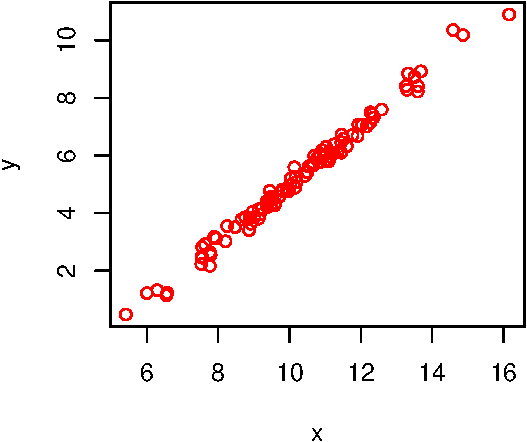
\includegraphics{Correlacion_files/figure-beamer/unnamed-chunk-1-1} 

}

\caption{Gráfico de dispersión de dos variables que se predicen mutuamente.}\label{fig:unnamed-chunk-1}
\end{figure}
\end{frame}

\begin{frame}{Representación gráfica}
\protect\hypertarget{representaciuxf3n-gruxe1fica-1}{}
\begin{figure}

{\centering 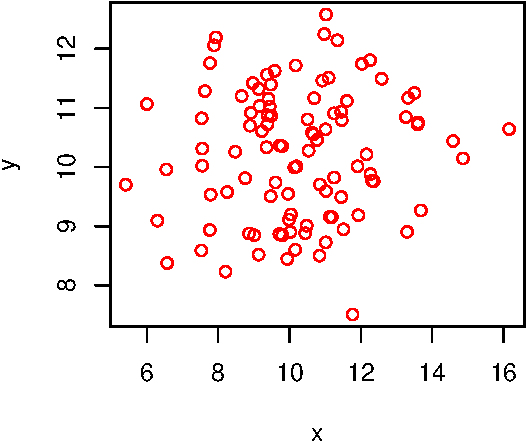
\includegraphics{Correlacion_files/figure-beamer/unnamed-chunk-2-1} 

}

\caption{Gráfico de dispersión de dos variables que no se predicen mutuamente.}\label{fig:unnamed-chunk-2}
\end{figure}
\end{frame}

\begin{frame}{Medición de la asociación}
\protect\hypertarget{mediciuxf3n-de-la-asociaciuxf3n}{}
\begin{itemize}
\item
  Prueba estadística por defecto:
  \href{https://en.wikipedia.org/wiki/Pearson_correlation_coefficient}{Coeficiente
  de correlación de Pearson}
\item
  Estima cociente de covarianza y producto de desviación estándar:
\end{itemize}

\begin{equation}
r_{X, Y} = \frac{\mathrm{cov}(X, Y)}{\sigma_{x} \sigma_{y}}
\end{equation}

\begin{equation}
\mathrm{cov}(X, Y) = \mathbb{E}[(X - \mu_x) (Y - \mu_y)]
\end{equation}
\end{frame}

\hypertarget{coeficiente-de-correlaciuxf3n-paso-a-paso}{%
\section{Coeficiente de correlación paso a
paso}\label{coeficiente-de-correlaciuxf3n-paso-a-paso}}

\begin{frame}{El caso no espacial}
\protect\hypertarget{el-caso-no-espacial}{}
Comenzamos con dos variables \(X\) y \(Y\):

\begin{longtable}[]{@{}rr@{}}
\caption{Primeras seis filas de tabla que contiene \emph{X} y
\emph{Y}.}\tabularnewline
\toprule()
x & y \\
\midrule()
\endfirsthead
\toprule()
x & y \\
\midrule()
\endhead
6.567783 & 8.377792 \\
9.385544 & 10.875437 \\
10.025123 & 8.902984 \\
9.477216 & 11.394629 \\
10.691021 & 11.163742 \\
11.768682 & 7.508639 \\
\bottomrule()
\end{longtable}
\end{frame}

\begin{frame}{Covarianza entre \(X\) y \(Y\)}
\protect\hypertarget{covarianza-entre-x-y-y}{}
\begin{equation}
\mathrm{cov}(X, Y) = \mathbb{E}[(X - \mu_x) (Y - \mu_y)]
\end{equation}

De adentro de paréntesis: - \(\mu_x =\) Promedio de \(X\); \(\mu_y =\)
Promedio de \(Y\)

\begin{itemize}
\item
  \(\mu_x = 10.23; \mu_y = 10.22\)
\item
  Restamos \(\mu\) de todos los valores de \(X\) y \(Y\)
\item
  \(X^*=X - \mu_x; Y^*=Y - \mu_y\)
\end{itemize}
\end{frame}

\begin{frame}{Covarianza entre \(X\) y \(Y\)}
\protect\hypertarget{covarianza-entre-x-y-y-1}{}
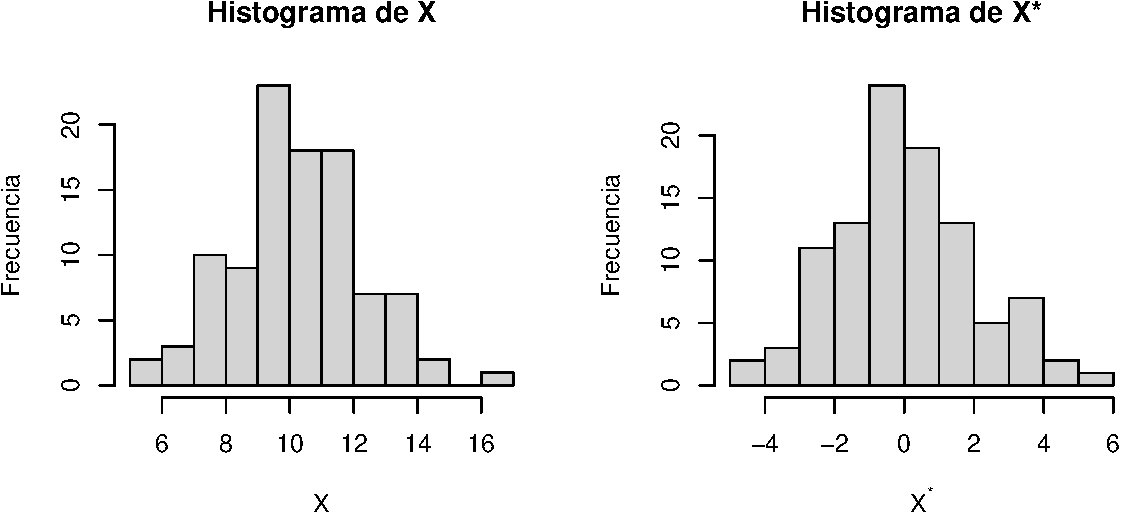
\includegraphics{Correlacion_files/figure-beamer/unnamed-chunk-4-1.pdf}
\end{frame}

\begin{frame}{Covarianza entre \(X\) y \(Y\)}
\protect\hypertarget{covarianza-entre-x-y-y-2}{}
Entonces las variables centradas quedan así:

\begin{longtable}[]{@{}rr@{}}
\caption{Variables \emph{X} y \emph{Y} centradas (con media de
0).}\tabularnewline
\toprule()
x & y \\
\midrule()
\endfirsthead
\toprule()
x & y \\
\midrule()
\endhead
-3.6683642 & -1.8473745 \\
-0.8506034 & 0.6502711 \\
-0.2110244 & -1.3221819 \\
-0.7589320 & 1.1694628 \\
0.4548737 & 0.9385757 \\
1.5325346 & -2.7165272 \\
\bottomrule()
\end{longtable}
\end{frame}

\begin{frame}{Covarianza entre \(X\) y \(Y\)}
\protect\hypertarget{covarianza-entre-x-y-y-3}{}
\begin{itemize}
\tightlist
\item
  Multiplicamos cada valor \(X^*_i\) por su correspondiente \(Y^*_i\)
\end{itemize}

\begin{align*}
X^*_1 \times Y^*_1 =  & -3.668 \times -1.847 = & 6.776 \\
X^*_2 \times Y^*_2 =  & -0.85 \times -0.65 = & -0.553 \\
X^*_3 \times Y^*_3 =  & -0.211 \times -1.322 = & 0.279 \\
\vdots
\end{align*}

\begin{itemize}
\tightlist
\item
  Terminamos haciendo: \(\frac{1}{n}\sum X^*_i Y^*_i\), es decir el
  promedio de los productos
\end{itemize}
\end{frame}

\begin{frame}{Producto de las desviaciones estándar}
\protect\hypertarget{producto-de-las-desviaciones-estuxe1ndar}{}
El denominador de la fórmula para la correlación es:

\begin{equation*}
\sigma_x \sigma_y
\end{equation*}

donde \(\sigma\) indica la desviación estándar de la variable en el
subíndice. Recordemos:

\begin{equation}
\sigma_x = \sqrt{\sum \frac{(X_i - \mu_x)^2}{n-1}}
\end{equation}
\end{frame}

\begin{frame}{Producto de las desviaciones estándar}
\protect\hypertarget{producto-de-las-desviaciones-estuxe1ndar-1}{}
Dado que ya contamos con \(X_i - \mu_x\) y \(Y_i - \mu_x\), sólo tenemos
que hacer \({X^*}^2\):

\begin{align*}
{X^*_1}^2 & = 6.776^2 = & 45.92 \\
{X^*_2}^2 & = -0.553^2 = & 0.305 \\
{X^*_3}^2 & = 0.279^2 = & 0.077 \\
\vdots
\end{align*}
\end{frame}

\begin{frame}{Producto de las desviaciones estándar}
\protect\hypertarget{producto-de-las-desviaciones-estuxe1ndar-2}{}
Una vez, obtenidos \({X^*}^2\) y \({Y^*}^2\), las sumamos y dividimos
entre \(n-1 = 99\):

\begin{align*}
\sum {X^*_i}^2/99 & = 391.1758/99 = 3.951\\
\sum {Y^*_i}^2/99 & = 119.9985/99 = 1.191
\end{align*}

Y terminamos sacando las raíces cuadradas:

\begin{align*}
\sqrt{9.951} & = 1.987\\
\sqrt{1.191} & = 1.091
1.987 \times 1.091 & = 2.17
\end{align*}
\end{frame}

\begin{frame}{Cálculo final de \(r\)}
\protect\hypertarget{cuxe1lculo-final-de-r}{}
Una vez obtenidos:

\begin{itemize}
\tightlist
\item
  \(\mathrm{cov}(X, Y) = 0.166\)
\item
  \(\sigma_x \sigma_y = 2.17\)
\end{itemize}

Tenemos:

\begin{equation*}
 \frac{\mathrm{cov}(X, Y)}{\sigma_x \sigma_y} = \frac{0.166}{2.17} = 0.091
\end{equation*}

\emph{El resultado no es preciso por varias operaciones que obviaron
decimales}
\end{frame}

\begin{frame}[fragile]{Prueba de correlación en \textbf{R}}
\protect\hypertarget{prueba-de-correlaciuxf3n-en-r}{}
\begin{itemize}
\item
  Función para hacer prueba \texttt{cor.test}
\item
  Uso:
\end{itemize}

\begin{Shaded}
\begin{Highlighting}[]
\FunctionTok{cor.test}\NormalTok{(x, y)}
\end{Highlighting}
\end{Shaded}

\begin{itemize}
\item
  \texttt{x} y \texttt{y} son las variables \(X\) y \(X\)

  \begin{itemize}
  \tightlist
  \item
    \textbf{Deben existir en el espacio de trabajo de R}
  \end{itemize}
\end{itemize}
\end{frame}

\begin{frame}[fragile]{Resultado de la prueba de correlación en
\textbf{R}}
\protect\hypertarget{resultado-de-la-prueba-de-correlaciuxf3n-en-r}{}
\begin{Shaded}
\begin{Highlighting}[]
\FunctionTok{cor.test}\NormalTok{(x, y)}
\end{Highlighting}
\end{Shaded}

\begin{verbatim}
## 
##  Pearson's product-moment correlation
## 
## data:  x and y
## t = 0.76948, df = 98, p-value = 0.4435
## alternative hypothesis: true correlation is not equal to 0
## 95 percent confidence interval:
##  -0.1207608  0.2698067
## sample estimates:
##       cor 
## 0.0774955
\end{verbatim}
\end{frame}

\begin{frame}[fragile]{Interpretación}
\protect\hypertarget{interpretaciuxf3n}{}
\begin{itemize}
\item
  \texttt{t\ =\ 0.76948}, valor del estadístico T-Student
\item
  \texttt{df\ =\ 98}, grados de libertad
\item
  \texttt{p-value\ =\ 0.4435}, probabilidad de que \(r = 0\)

  \begin{itemize}
  \tightlist
  \item
    Probabilidad de que la correlación no exista
  \end{itemize}
\item
  \texttt{cor\ 0.0774955}, valor del coeficiente de correlación estimado
\end{itemize}
\end{frame}

\begin{frame}{Limitaciones - Ejemplo}
\protect\hypertarget{limitaciones---ejemplo}{}
Relación entre poblaciones de mariposas, toneladas de pesticida y
televisiones (Reino Unido)

\begin{itemize}
\item
  Toneladas de pesitida en aumento
\item
  Densidad de mariposas disminuye
\item
  Cantidad de licencias de televisión en aumento
\end{itemize}
\end{frame}

\begin{frame}{Limitaciones - Gráficos}
\protect\hypertarget{limitaciones---gruxe1ficos}{}
Densidad de mariposas

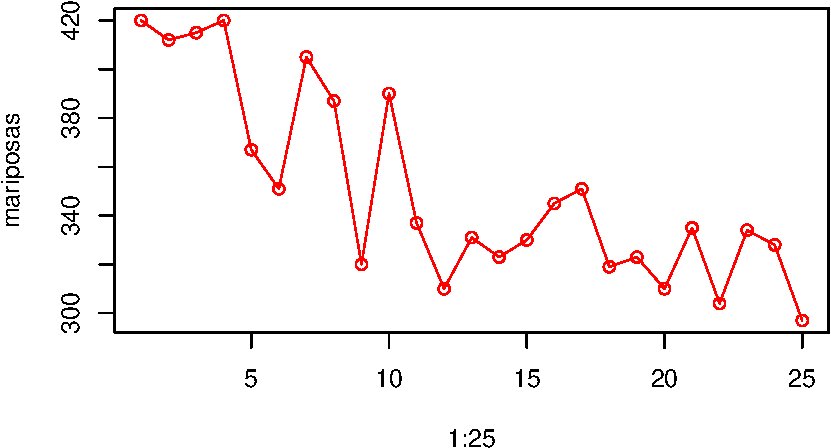
\includegraphics{Correlacion_files/figure-beamer/unnamed-chunk-8-1.pdf}
\end{frame}

\begin{frame}{Limitaciones - Gráficos}
\protect\hypertarget{limitaciones---gruxe1ficos-1}{}
Uso de pesticidas

\begin{figure}
\centering
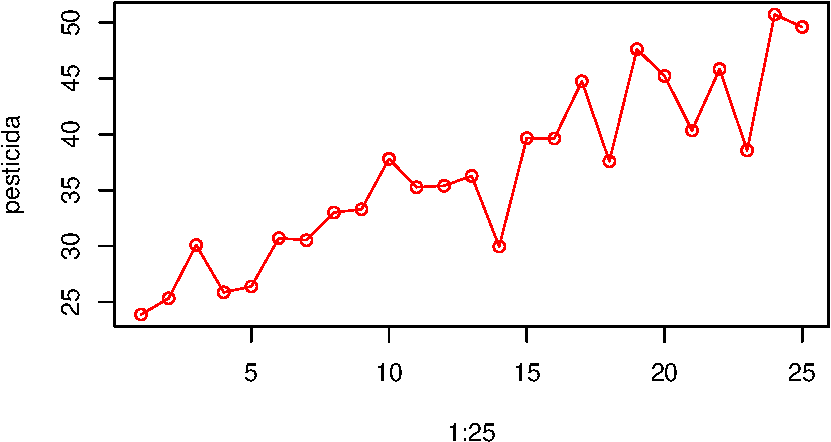
\includegraphics{Correlacion_files/figure-beamer/unnamed-chunk-9-1.pdf}
\caption{Porcentaje de área cubierta con pesticida.}
\end{figure}
\end{frame}

\begin{frame}{Limitaciones - Gráficos}
\protect\hypertarget{limitaciones---gruxe1ficos-2}{}
\begin{figure}
\centering
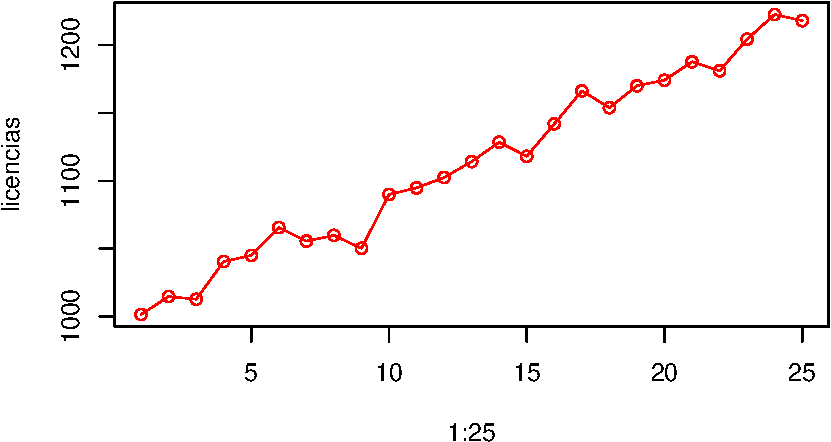
\includegraphics{Correlacion_files/figure-beamer/unnamed-chunk-10-1.pdf}
\caption{Número mensual promedio de licencias de televisión vendidas.}
\end{figure}
\end{frame}

\begin{frame}{Limitaciones - Correlaciones entre variables}
\protect\hypertarget{limitaciones---correlaciones-entre-variables}{}
\begin{center}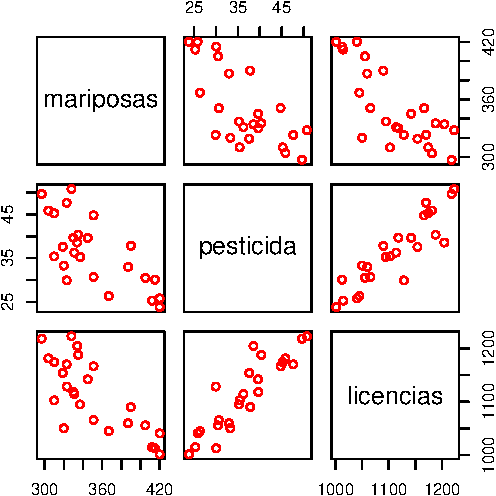
\includegraphics{Correlacion_files/figure-beamer/unnamed-chunk-11-1} \end{center}
\end{frame}

\begin{frame}{Limitaciones - Coeficientes de correlación}
\protect\hypertarget{limitaciones---coeficientes-de-correlaciuxf3n}{}
\begin{longtable}[]{@{}lrrr@{}}
\caption{Matriz de correlación entre todas las
variables.}\tabularnewline
\toprule()
& mariposas & pesticida & licencias \\
\midrule()
\endfirsthead
\toprule()
& mariposas & pesticida & licencias \\
\midrule()
\endhead
mariposas & 1.0000000 & -0.7143064 & -0.7764724 \\
pesticida & -0.7143064 & 1.0000000 & 0.8986094 \\
licencias & -0.7764724 & 0.8986094 & 1.0000000 \\
\bottomrule()
\end{longtable}
\end{frame}

\begin{frame}{Limitaciones - Conclusiones}
\protect\hypertarget{limitaciones---conclusiones}{}
La venta de licencias de televisión mata a las mariposas
\end{frame}

\begin{frame}{Limitaciones - Conclusiones}
\protect\hypertarget{limitaciones---conclusiones-1}{}
\begin{itemize}
\item
  La correlación no mide causa y efecto
\item
  Correlación puede ocurrir al azar
\item
  Sólo sirve para medir asociación
\item
  Interpretación de asociación \(\rightarrow\) Conocimiento del fenómeno
  estudiado

  \begin{itemize}
  \tightlist
  \item
    Es más probable que, aunque la correlación sea menor, la
    discminución sea producto del uso de pesticidas
  \end{itemize}
\end{itemize}
\end{frame}

\end{document}
